\documentclass{article}

\usepackage{graphicx}
\usepackage{tikz}
\usepackage{tikzsymbols}
\usetikzlibrary{calc,patterns,shapes.geometric}
\pagestyle{empty}
\usepackage[margin=0pt]{geometry}
\geometry{papersize={14in,12in}}

\def\centerarc[#1](#2)(#3:#4:#5){\draw[#1] ($(#2)+({#5*cos(#3)},{#5*sin(#3)})$) arc (#3:#4:#5);}

\begin{document}
	\begin{figure}
		\centering
		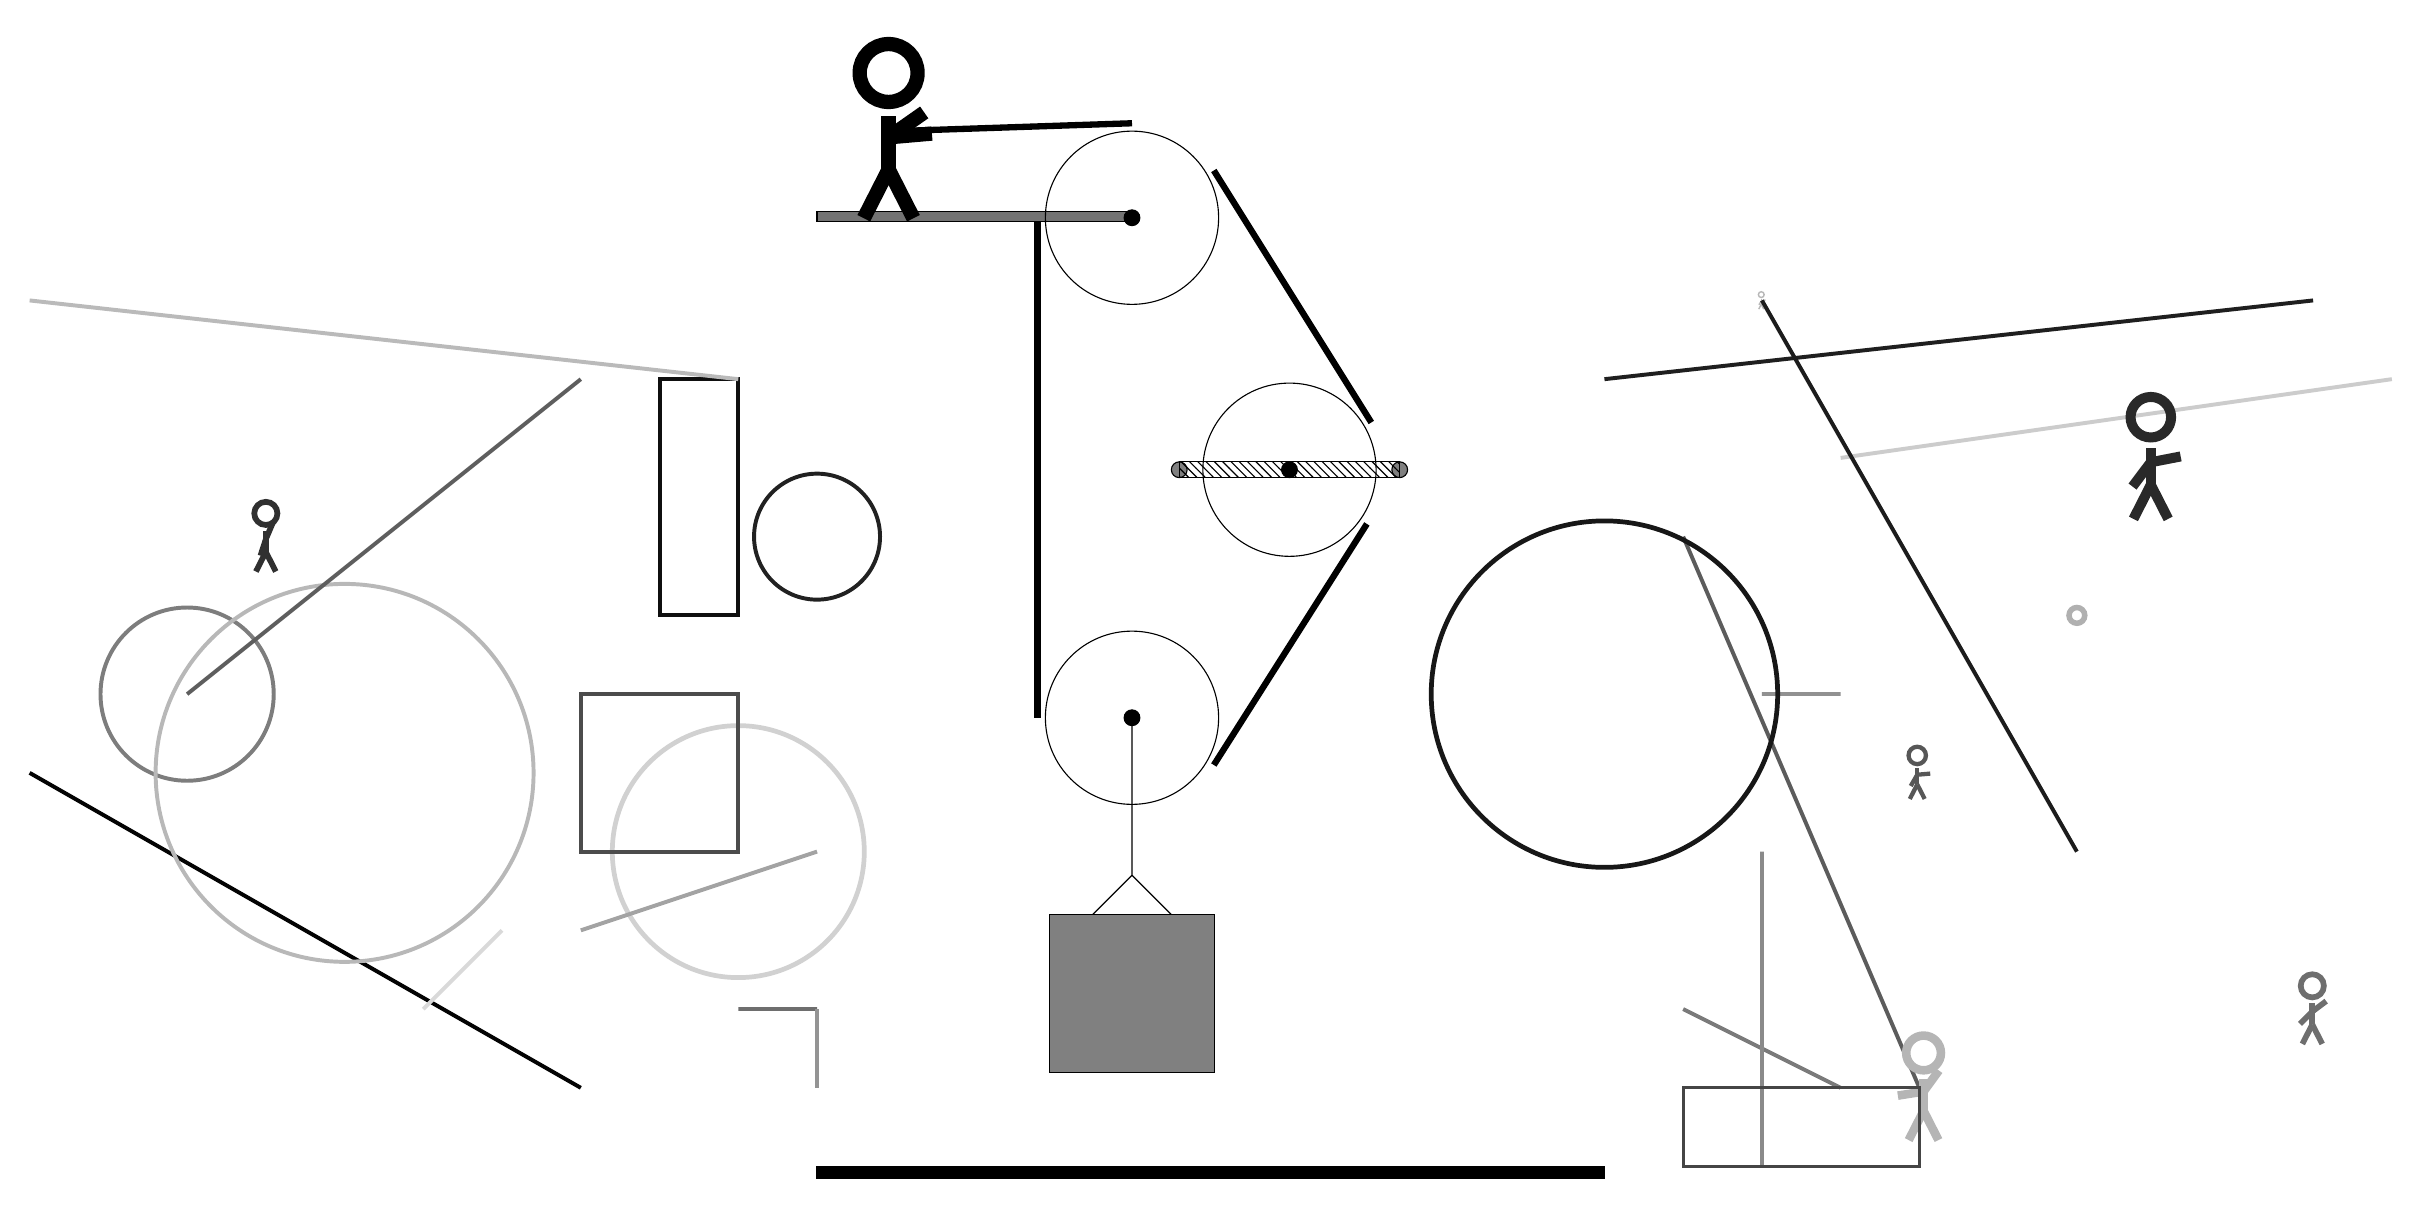
\begin{tikzpicture}
			%%%%% START %%%%%
			
			\draw[fill=black!55] (-2, 9) rectangle (2, 9.125);
			
			\draw (2, 2.7) circle (1.1);
			\draw[fill=black] (2, 2.7) circle (0.1);
			
			\draw (2, 9.05) circle (1.1);
			\draw[fill=black] (2, 9.05) circle (0.1);
			
			\draw[fill=white](4, 5.85) circle (1.1);
			\draw[fill=black] (4, 5.85) circle (0.1);
			\draw[fill=black!50] (2.6, 5.85) circle (0.1);
			\draw[fill=black!50] (5.4, 5.85) circle (0.1);
			\draw[pattern=north west lines, pattern color=black] (2.6, 5.95) rectangle (5.4, 5.75);
			
			\draw[line width=0.5mm, color=black!20](11, 6) -- (18, 7);
			
			\draw [line width=0.6mm, color=black!18](-3, 1) circle (1.6);
			\node[line width=0.7mm, color=black!81] at (-9, 5) {\Strichmaxerl[4][72][67]};
			\draw [line width=0.5mm, color=black!87](-2, 5) circle (0.8);
			\draw[line width=0.5mm, color=black!52](9, -1) -- (11, -2);
			\draw[line width=0.5mm, color=black!70] (-3, 1) rectangle (-5, 3);
			\draw[line width=0.5mm, color=black!64](9, 5) -- (12, -2);
			\draw[line width=0.6mm, color=black!57] (-2, -1) rectangle (-3, -1);
			\draw[line width=0.5mm, color=black!99](-5, -2) -- (-12, 2);
			\draw[line width=0.5mm, color=black!94] (-4, 7) rectangle (-3, 4);
			\draw[line width=0.5mm, color=black!43] (10, 3) rectangle (11, 3);
			\draw[line width=0.5mm, color=black!27](-3, 7) -- (-12, 8);
			\draw [line width=0.5mm, color=black!51](-10, 3) circle (1.1);
			\draw [line width=0.5mm, color=black!28](-8, 2) circle (2.4);
			\node[line width=0.3mm, color=black!57] at (17, -1) {\Strichmaxerl[4][45][37]};
			\draw[line width=0.5mm, color=black!63](-5, 7) -- (-10, 3);
			
			\draw[line width=0.5mm, color=black!88](8, 7) -- (17, 8);
			
			\draw[line width=0.5mm, color=black!15](-6, 0) -- (-7, -1);
			\draw[line width=0.6mm, color=black!42] (-2, -2) rectangle (-2, -1);
			\draw[line width=0.5mm, color=black!46] (10, 1) rectangle (10, -3);
			\node[line width=0.7mm, color=black!29] at (12, -2) {\Strichmaxerl[6][9][54]};
			
			\draw[line width=0.4mm, color=black!73] (9, -3) rectangle (12, -2);
			\node[line width=0.5mm, color=black!84] at (15, 6) {\Strichmaxerl[7][53][11]};
			\draw [line width=0.7mm, color=black!31](14, 4) circle (0.1);
			\node[line width=0.6mm, color=black!66] at (12, 2) {\Strichmaxerl[3][60][5]};
			\draw [line width=0.6mm, color=black!91](8, 3) circle (2.2);
			\node[line width=0.7mm, color=black!28] at (10, 8) {\Strichmaxerl[1][58][15]};
			\draw[line width=0.5mm, color=black!36](-5, 0) -- (-2, 1);
			\draw[line width=0.5mm, color=black!89](10, 8) -- (14, 1);
			
			\draw (2, 2.7) -- (2, 0.7) -- (1.5, 0.2) -- (2.5, 0.2) -- (2, 0.7);
			\draw[fill=black!50] (0.95, 0.2) rectangle (3.05, -1.8);
			
			\draw[line width=0.8mm] (0.8, 9) -- (0.8, 2.7);
			\centerarc[line width=0.8mm](2, 2.7)(180:330:1.2000000000000002);
			\draw[line width=0.8mm](3.0392, 2.1) -- (4.983, 5.1617);
			\centerarc[line width=0.8mm](4, 5.85)(390:325:1.2000000000000002);
			\draw[line width=0.8mm](5.0392, 6.45) -- (3.0392, 9.65);
			\centerarc[line width=0.8mm](2, 9.05)(30:90:1.2000000000000002);
			\draw[line width=0.8mm](2, 10.25) -- (-1, 10.15);
			
			\node at (-1, 10.15) {\Strichmaxerl[10][-175][35]};
			
			\draw[fill=black] (-2, -3) rectangle (8, -3.15);
			
			%%%%% END %%%%%
		\end{tikzpicture}
	\end{figure}	
\end{document}